% Copyright 2012 Bruno Menegola
%
% This work may be distributed and/or modified under the
% conditions of the LaTeX Project Public License, either version 1.3
% of this license or (at your option) any later version.
% The latest version of this license is in
%   http://www.latex-project.org/lppl.txt
% and version 1.3 or later is part of all distributions of LaTeX
% version 2005/12/01 or later.
%
% This work has the LPPL maintenance status ‘maintained’.
%
% The Current Maintainer of this work is Bruno Menegola.
%
% This work consists of all files listed in MANIFEST
%
%
% Description
% ===========
%
% This is an example latex document to build presentation slides based on
% the beamer class using the Inf theme.

\documentclass{beamer}

\usepackage[T1]{fontenc}
\usepackage[brazil]{babel}
\usepackage[utf8]{inputenc}
\usepackage{bookmark}

\graphicspath{ {./images/} }

% Choose the Inf theme
\usetheme{Inf}

% Define the title with \title[short title]{long title}
% Short title is optional
\title[BNN]
      {Bayesian Neural Networks: An Introduction and Survey}

% Optional subtitle
\subtitle{Estatítica Computacional}

\date{Agosto de 2025}

% Author information
\author{Eduardo Azeredo}
\institute{Faculdade de Ciências Econômicas --- UFRGS\\\texttt{ufrgs.br/fce}}

\begin{document}

% Command to create title page
\InfTitlePage

% \begin{frame}
%   \frametitle{Agenda}
%   \tableofcontents
% \end{frame}

\section{Introdução}

\frame{
    \frametitle{Redes Neurais - Função de Ativação}

    \begin{columns}[c] % "c" means vertically centered
        \begin{column}{0.55\textwidth}
            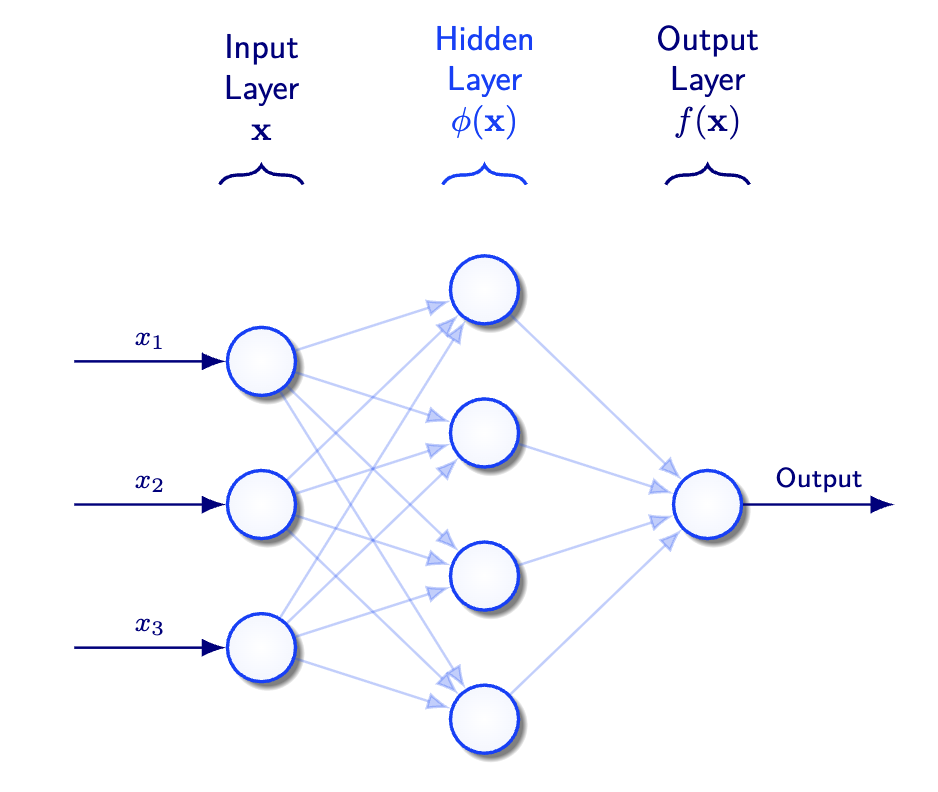
\includegraphics[width=\linewidth]{nn_diagram.png} % replace with your image
        \end{column}
        \begin{column}{0.45\textwidth}
            % \begin{itemize}
                % \item
                Podemos representar uma rede neural como uma função:
                $$ \phi_j = \sum^{N_1}_{i=1} a(x_iw^1_{ij}) $$
                onde $a$ é uma função de ativação.
            % \end{itemize}
        \end{column}
    \end{columns}
    % 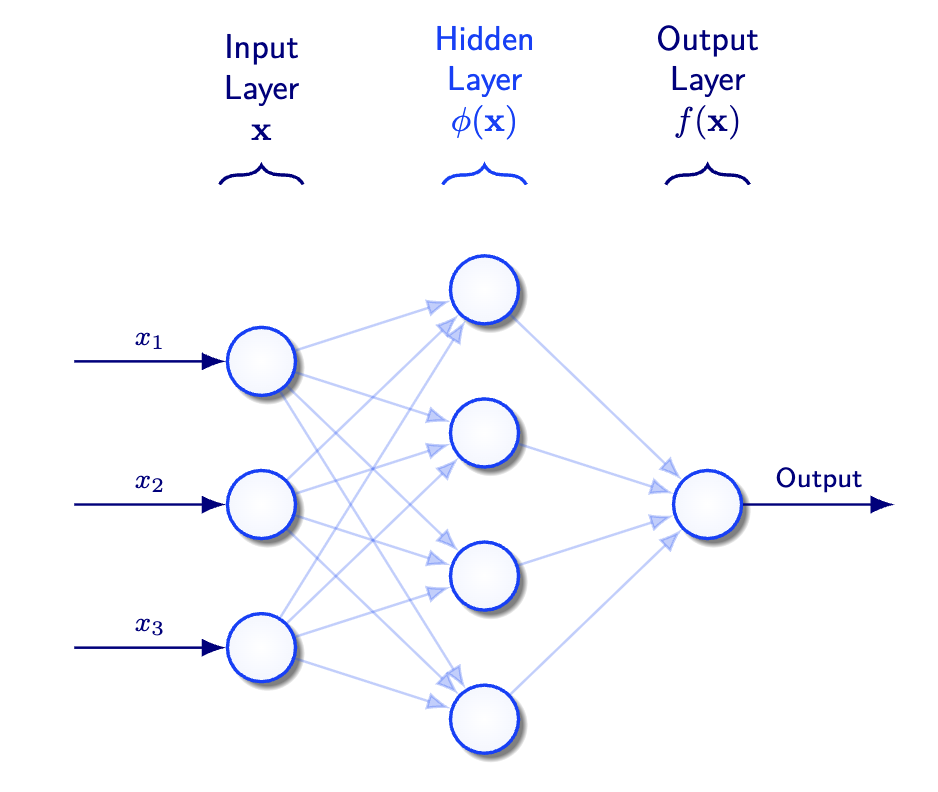
\includegraphics[scale=0.5]{nn_diagram.png}
}

\frame{
    \frametitle{Redes Neurais - Output}

    \begin{columns}[c] % "c" means vertically centered
        \begin{column}{0.55\textwidth}
            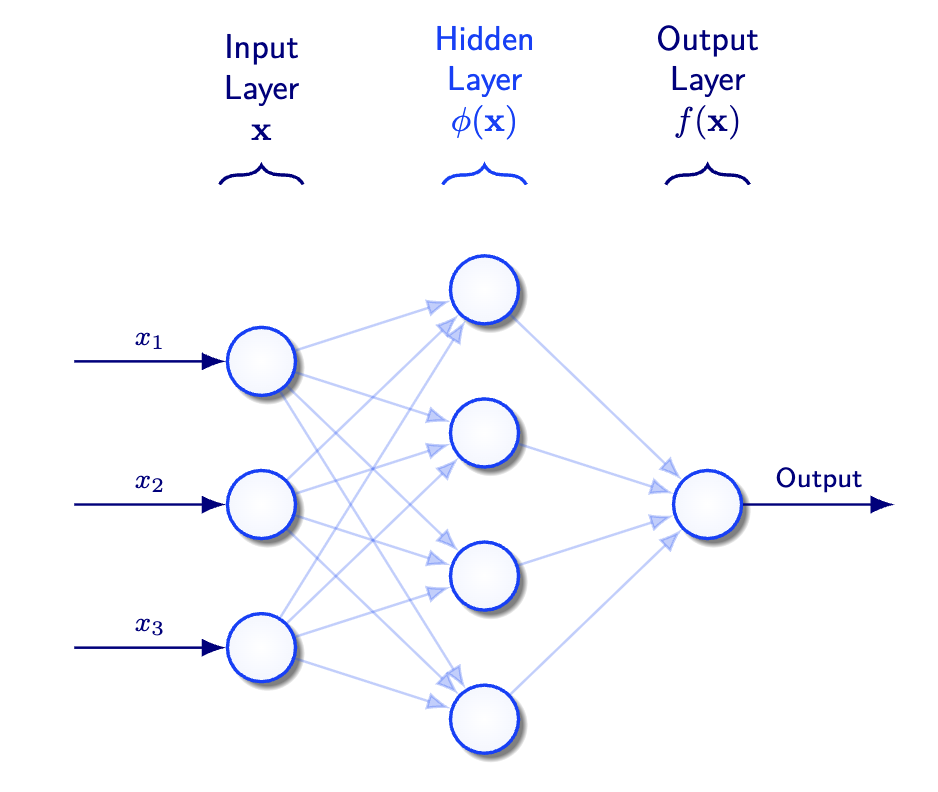
\includegraphics[width=\linewidth]{nn_diagram.png} % replace with your image
        \end{column}
        \begin{column}{0.45\textwidth}
            % \begin{itemize}
                % \item
                A saída da rede neural é dada por:
                $$ f_k = \sum^{N_2}_{j=1} g(\phi_jw^2_{ik}) $$
                onde $g$ ou é a função identidade (regressão) ou uma função softmax (classificação).
            % \end{itemize}
        \end{column}
    \end{columns}
    % 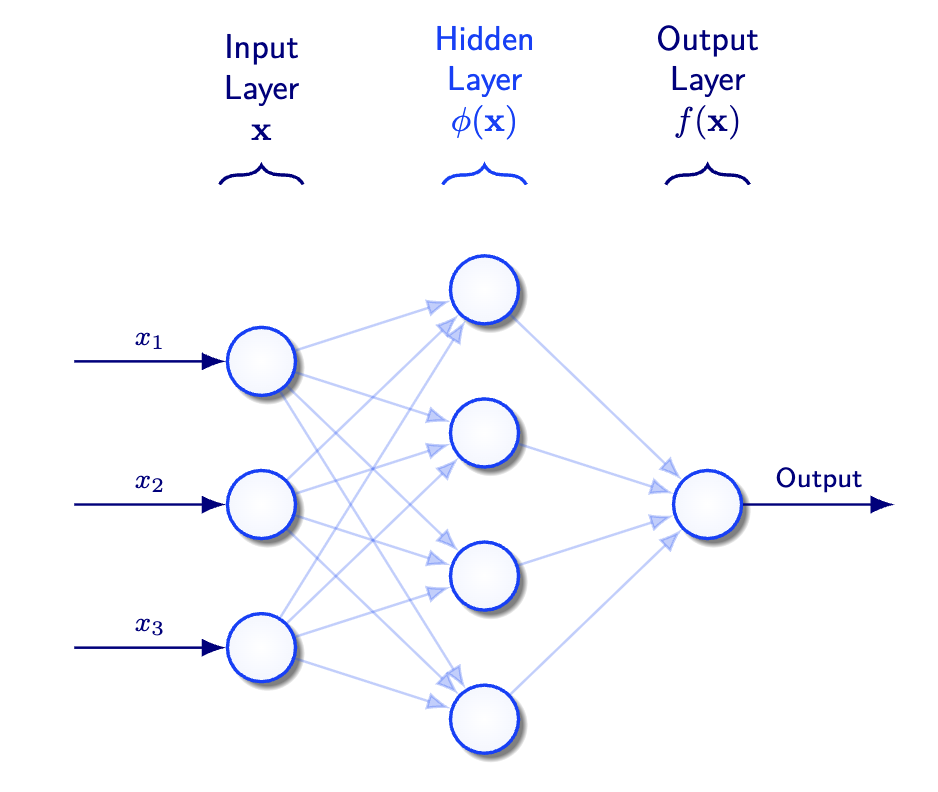
\includegraphics[scale=0.5]{nn_diagram.png}
}

\frame{
    \frametitle{Redes Neurais - Treinamento}

    \begin{itemize}
        \item O treinamento da rede consiste em achar os pesos $\mathbf{w}$ que melhor aproximam a função desejada;
        \item A minimização é feita via descida de gradiente, calculando os gradiente em relação aos pesos;
        \item Esse processo é conhecido como backpropagation.
        \item Em termos estatísticos, os pesos $\mathbf{w}$ são os parâmetros desconhecidos do modelo, e o treinamento é o processo de estimá-los. \textbf{Esta é uma abordagem frequentista}.
    \end{itemize}
}

\section{Redes Neurais Bayesianas}

\begin{frame}
    \frametitle{História}

    \begin{itemize}
        \item Tishby, Levin e Solla (1989), ao estudar as propriedades estatísticas de NN, mostraram que atribuir um prior aos pesos pode ser usado para gerar uma posterior, sem indicar como obtê-la;
        \item Denker e LeCun (1991) propõe um método usando aproximação de Laplace para calcular a posterior;
        \item Hinton e Van Camp (1993) propõem o uso de Inferência Variacional (VI) para aproximar a posterior;
        \item Neal (1996) propõe o uso de MCMC para amostrar a posterior usando Hybrid/Hamiltonian Monte Carlo (HMC);
    \end{itemize}

\end{frame}

\frame{
    \frametitle{Redes Neurais Bayesianas - Introdução}

    \begin{itemize}
        \item Se atribuirmos que os pesos $\mathbf{w}$ são variáveis aleatórias, e que podemos atribuir uma distribuição a eles, temos uma rede neural bayesiana;
        \item Normalmente atribuímos uma distribuição normal centrada em $0$ com baixa variância aos pesos, isso é uma constatação empírica; vale então o Teorema de Bayes
        $$ \pi(\mathbf{w}|\mathcal{D}) = \frac{p(\mathbf{w})p(\mathcal{D}|\mathbf{w})}{\int p(\mathbf{w})p(\mathcal{D}|\mathbf{w}) d\mathbf{w}} = \frac{p(\mathbf{w})p(\mathcal{D}|\mathbf{w})}{p(\mathcal{D})} $$
        \item Onde $\mathcal{D}$ é o conjunto de dados, $p(\mathbf{w})$ é a distribuição a priori dos pesos, $p(\mathcal{D}|\mathbf{w})$ é a verossimilhança dos dados, $\pi(\mathbf{w}|\mathcal{D})$ é a distribuição posterior verdadeira dos pesos, e $p(\mathcal{D})$ é a evidência.
    \end{itemize}
}

\begin{frame}
    \frametitle{}

    \begin{itemize}
        \item A predição desse modelo é dada por:
        $$ \mathbb{E}_\pi (\mathbf{w}) = \int f(\mathbf{w})\pi(\mathbf{w}|\mathcal{D}) d\mathbf{w} $$
        \item "opposed to an optimisation scheme used in the frequentist setting [...] our predictions are represented in the form of valid conditional probabilities";
        \item O problema é que, mesmo para problemas simples, não conseguimos calcular a integral. Para isso usamos métodos de aproximação, sendo o mais comum VI, ou Variational Inference.
    \end{itemize}
\end{frame}

\section{Método de aproximação}

\subsection{Inferência Variacional}

\frame{
    \frametitle{Introdução}

    \begin{itemize}
        \item A ideia central da VI é transformar o problema de inferência em um problema de otimização;
        \item Assumimos uma distribuição $q_\theta(\mathbf{w})$ e através usando divergência Kullback-Leibler (KL) aproximamos a posterior verdadeira $\pi(\mathbf{w}|\mathcal{D})$; Definimos primeiro divergência KL
        $$ KL[q_\theta(\mathbf{w}) || p(\mathbf{w}|p(\mathbf{w}|\mathcal{D}))] = \int q_\theta(\mathbf{w}) \log\left(\frac{q_\theta(\mathbf{w})}{p(\mathbf{w}|\mathcal{D})}\right) d\mathbf{w} $$
        \item Podemos então minimizar a divergência KL em relação aos parâmetros $\theta$:
        $$ \theta^* = \arg\min_\theta KL[q_\theta(\mathbf{w}) || p(\mathbf{w}|\mathcal{D})] $$
    \end{itemize}
}

\begin{frame}
    \frametitle{ELBO}

    Podemos expandir a expressão da divergência KL como
    \begin{align*}
        KL[q_\theta(\mathbf{w}) || p(\mathbf{w}|\mathcal{D})] &= \mathbb{E}_q \left(\log \frac{q_\theta(\mathbf{w})}{p(\mathbf{w})} - \log p(\mathbf{w}|\mathcal{D}) \right) + \log p(\mathcal{D})
        \\&= KL\left( q_\theta(\mathbf{w}||p(\mathbf{w})) \right) - \mathbb{E}_q \left[\log p(\mathcal{D}|\mathbf{w})\right] + \log p(\mathcal{D})
        \\&= - \mathcal{F}[q_\theta] + \log p(\mathcal{D})
    \end{align*}
    Onde $\mathcal{F}[q_\theta] = - KL\left( q_\theta(\mathbf{w}||p(\mathbf{w})) \right) + \mathbb{E}_q \left[\log p(\mathcal{D}|\mathbf{w})\right]$, que depende somente de componentes conhecidos. Não somente, o termo $\log p(\mathcal{D})$ é constante em relação a $\theta$, e pode ser ignorado na otimização. Temos então o novo problema de otimização:
    $$ \theta^* = \arg\max_\theta -\mathcal{F}[q_\theta] $$
\end{frame}


\begin{frame}
    \frametitle{Limitações}

    Até então os resultados apresentados se restringem a uma NN com apenas uma camada escondida e possuem certas desvantagens:
    \begin{itemize}
        \item A distribuição tem que ser possível de ser fatorizada entre os pesos o que sacrifica a capacidade dos pesos de demonstrar correlações;
        \item Barber e Bishop (1998) estendem o domínio do problema para permitir correlações usando uma distribuição gaussiana multivariada, mas isso aumenta o número de parâmetros a serem otimizados;
        \item A função de ativação deve ser sigmóide que tem um gradiente que pode resultar em baixa performance no aprendizado.
    \end{itemize}
\end{frame}

\begin{frame}
    \frametitle{Soluções}

    \begin{itemize}
        \item Welling e Teh (2011) propões o uso de mini-batches e SGD para otimizar a ELBO;
        \item Graves (2011) propõem o uso de MFVB, alterando a função $\mathcal{F}[q_\theta]$ como a soma de duas esperanças que podem ser resolvidas via integração Monte Carlo para achar os gradientes;
        $$ \mathcal{F}[q_\theta] = \mathbb{E}_q [\log(p(\mathcal{D}|\mathbf{w}))] - \mathbb{E}_q [\log(p_\theta(\mathbf{w})) - \log(p(\mathbf{w}))] $$
        \item Kingma e Welling (2014) propõem o uso do "truque de reparametrização" para reduzir a variância da estimação dos gradientes;
    \end{itemize}
\end{frame}

\begin{frame}
    \frametitle{Dropout como VI}

    Gal (2016) propõe o uso de Dropout (um método de regularização) para introduizr estocasticidade nos parâmetros de uma rede neural.
    \begin{align*}
        \mathbf{W}^1_\rho &= diag(\rho)\mathbf{W}^1
        \\ \Phi_\rho &= a(\mathbf{X}^T\mathbf{W}^1_\rho)
    \end{align*}
    onde $\rho$ é um vetor de uma Bernoulli($p$) e $diag(\rho)$ é uma matriz diagonal com os elementos de $\rho$ na diagonal. Dessa forma preservamos alguma correlação entre os parâmetros.
    A posterior aproximada é então dada por uma Bernoulli multiplicada pelos pesos da rede.
\end{frame}

% \begin{frame}
%     \frametitle{Bayes by Backprop}

%     \begin{itemize}
%         \item Blundell et al. (2015) propõem o método Bayes by Backprop (BBB) que usa o truque de reparametrização para uma estimativa não viesada da esperança;
%         \item Assumimos uma distribuição normal para os pesos, ou seja, $q_\theta(\mathbf{w}) = \mathcal{N}(\mu, \sigma^2)$;
%         \item A amostra dos pesos é dada por $\mathbf{w} = \mu + \sigma \odot \epsilon$, onde $\epsilon \sim \mathcal{N}(0, I)$;
%         \item A ELBO é então dada por
%         $$ \mathcal{F}(\mathcal{D}, \theta) \approx \sum^{n}_{i=1} \log q_\theta(\mathbf{w}^{(i)}) - \log p(\mathbf{w}^{(i)}) - \log p(\mathcal{D}|\mathbf{w}^{(i)}) $$
%         onde $\mathbf{w}^{(i)}$ são amostras de $q_\theta(\mathbf{w})$;
%         \item A verossimilhança é normalmente fatorizada em mini-batches para reduzir o custo computacional;
%         \item A prior pode ser uma mistura de gaussianas para induzir sparsidade nos pesos
%     \end{itemize}
    
% \end{frame}

\subsection{Métodos de MCMC}

\frame{
    \frametitle{Introdução}

    \begin{itemize}
        \item Neal (1996) propõe o uso de MCMC para amostrar a posterior usando Hybrid/Hamiltonian Monte Carlo (HMC) e achar diretamente os momentos da predição;
        \item Originalmente da física estatística, HMC é um método que usa conceitos de mecânica hamiltoniana para propor novos estados de uma cadeia de Markov;
        \item HMC é um método de MCMC que usa o gradiente da função alvo para guiar a amostragem;
        \item O método é eficiente para problemas de alta dimensão, como é o caso das BNNs.
    \end{itemize}
}

\begin{frame}
    \frametitle{HMC}

    \begin{itemize}
        \item HMC introduz uma variável auxiliar $\mathbf{p}$, chamada de momento, e define a função energia hamiltoniana como
        $$ H(\mathbf{w}, \mathbf{p}) = U(\mathbf{w}) + K(\mathbf{v}) $$
        onde $U(\mathbf{w}) = -\log \left[ \pi(\mathbf{w}) \mathcal{L}(\mathbf{w}) \right]$ é a energia potencial e $K(\mathbf{m}) = \sum_{i=1}^{d}\frac{v_i^2}{2m_i}$ é a energia cinética. A distribuição conjunta é então dada por
        $$ p(\mathbf{w}, \mathbf{v}) = \frac{1}{Z} \exp (-U(\mathbf{w})) \exp (-K(\mathbf{v})) $$
        \item $K(\bf{v})$ é normalmente assumida como tendo uma distribuição normal centrada em $m$.
    \end{itemize}

\end{frame}


\begin{frame}
    \frametitle{Algoritmo}

    O algoritmo HMC é dado por:
    \begin{itemize}
        \item Inicializamos os pesos $\mathbf{w}$ e o momento $\mathbf{m}$;
        \item Amostramos da distribuição canônica de $H(\mathbf{w}, \mathbf{m})$
        \item Metropolis-Hastings:
        \begin{itemize}
            \item Simulamos a dinâmica hamiltoniana por um tempo $L$ com passos de tamanho $\epsilon$ usando o método leapfrog resultando em $(\mathbf{w}^*, \mathbf{m}^*)$;
            \item Calculamos a razão $r$ de aceitação
            $$ r = \frac{\mathcal{L}(\bf{w}^*) p(\bf{w}^*) \mathcal{N}(\bf{w}^*)}{\mathcal{L}(\bf{w}) p(\bf{w}) \mathcal{N}(\bf{w})} $$
            \item Aceitamos a proposta se $u \sim U(0,1) < r$, caso contrário mantemos o estado atual.
        \end{itemize}
    \end{itemize}

\end{frame}

\begin{frame}
    \frametitle{Ilustração}

    \begin{figure}[h]
        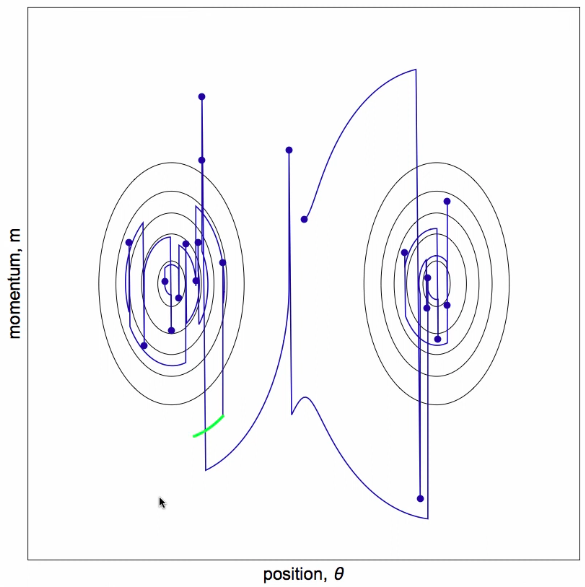
\includegraphics[scale=0.35]{hmc.png} % replace with your image
    \end{figure}

\end{frame}

% \begin{frame}
%     \frametitle{Fine-Tuning}

%     \begin{itemize}
%         \item $\epsilon$ e $L$ são hiperparâmetros do modelo que influenciam na eficiência do algoritmo;
%     \end{itemize}

% \end{frame}

\section{Comparação dos métodos}

\begin{frame}
    \frametitle{Métodos VI}

    \begin{columns}[c] % "c" means vertically centered
        \begin{column}{0.75\textwidth}
            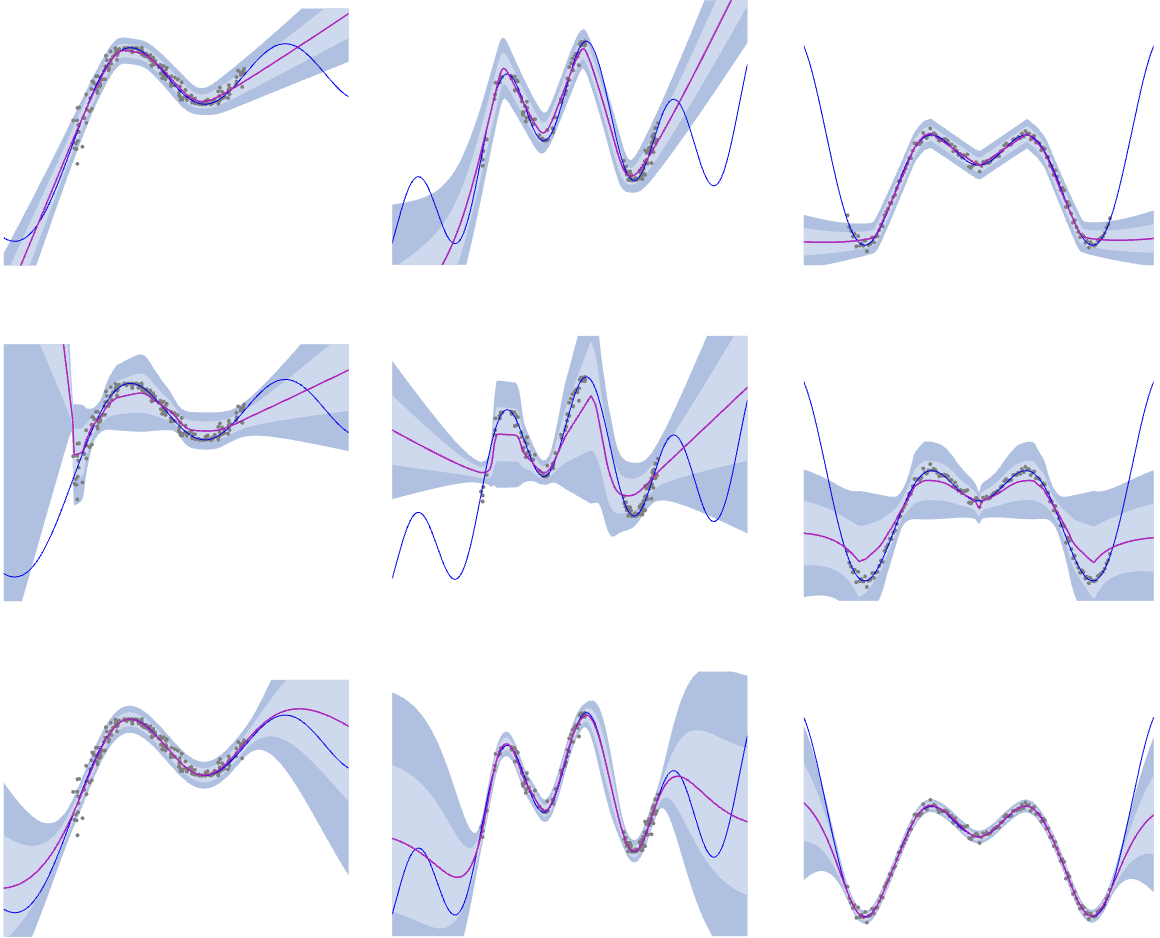
\includegraphics[width=\linewidth]{compare.png} % replace with your image
        \end{column}
        \begin{column}{0.25\textwidth}
            Primeira linha: VI (BBB)
            \break

            Segunda linha: VI MC Dropout
            \break

            Terceira linha: Processo Gaussiano
        \end{column}
    \end{columns}

\end{frame}

\section{Conclusão}

\begin{frame}
    \frametitle{Considerações Finais}

    \begin{itemize}
        \item BNNs tendem a subestimar a variância das predições, mesmo que as médias sejam acuradas;
        \item Muito da pesquisa em BNNs hoje ainda depende de métodos de VI por causa da facilidade de adaptá-lo à backpropagation;
        \item O uso da divergência KL permite separar a verossimilhança marginal da nossa função objetivo que permite um "alvo" para a otimização, só que KL não é um medida de distância, e sim de divergência, o uso de uma distância (Hellinger) pode se mostrar vantajoso, mas a dificuldade de definir uma função objetivo viável é um desafio;
        \item MCMC é computacionalmente custoso e métodos de sub-sampling se mostraram ineficientes em estimar uma posterior.
    \end{itemize}

\end{frame}


% \section{Detalhes}

% \frame{
%     \frametitle{História}

%     \begin{itemize}
%         \item O Instituto de Informática mudou de logotipo quando completou 20 anos
%         \item Entretanto os templates para slides continuaram os mesmos
%         \item Um manual de identidade visual veio junto com o artigo
%         \item Esse template que você vê é baseado nele
%     \end{itemize}
% }

% \frame{
%     \frametitle{Listas}

%     \begin{enumerate}
%         \item Listas não numeradas você já viu no slide anterior
%         \item Listas numeradas também são possíveis
%         \begin{itemize}
%             \item Assim como ambos os tipos em vários níveis
%         \end{itemize}
%     \end{enumerate}
% }

% \section{Outra seção}
% \subsection{Primeira subseção}

% \frame{
%     \frametitle{Seções}

%     \begin{itemize}
%         \item O número a esquerda do cabeçalho marca a seção atual
%         \item Logo a direita ele é seguido por:
%         \begin{itemize}
%             \item nome da seção
%             \item subseção
%             \item título do slide
%         \end{itemize}
%     \end{itemize}
% }

% \section{Blocos}

% \begin{frame}[plain]
%  \sectionpage
% \end{frame}

% \frame{
%     \frametitle{Teoremas}

%     \begin{theorem}
%         foo
%     \end{theorem}
%     \begin{proof}
%         bar
%     \end{proof}
% }

% \frame{
%     \frametitle{Exemplos}

%     \begin{exampleblock}{exemplo}
%         foo
%     \end{exampleblock}
% }

% \frame{
%     \frametitle{Alertas}

%     \begin{alertblock}{alerta}
%         foo
%     \end{alertblock}
% }

\section*{}

\frame{
    \frametitle{Referências}

    \begin{itemize}
        \item GOAN, Ethan; FOOKES, Clinton. Bayesian Neural Networks: An Introduction and Survey. In: [S.l.: S.n.]. v. 2259 p. 45-87. Disponível em: \url{http://arxiv.org/abs/2006.12024}. Acesso em: 25 ago. 2025.
        \item NEAL, Radford M. MCMC using Hamiltonian dynamics. [S.l.: S.n.]. Disponível em: \url{https://arxiv.org/pdf/1206.1901}. Acesso em: 2 set. 2025.
        \item The intuition behind the Hamiltonian Monte Carlo algorithm. Ben Lambert, 15 maio 2018. Disponível em: <\url{https://www.youtube.com/watch?v=a-wydhEuAm0}>. Acesso em: 2 set. 2025.
    \end{itemize}
}

\begin{frame}
    \frametitle{Obrigado!}
    \InfContacts
\end{frame}

\end{document}
